\chapter{Preliminary Study}

\renewcommand{\chaptername}{Chapter}

In this chapter, we start by studying the state of the art and we present the most important concepts evoked in  our project. Then we study the existing solution by defining its efficiency and its imperfections. Afterwards, we present our own additional provision.



%----------------------------------------------State of the art
\section{State of the art}

To be able to develop our project, a state of art study is in order. It helps understand the frameworks surrounding the new technologies that will be used to accomplish this work.

We devote this part to explain IT terms as well as the architecture of an Network security monitoring toolkit along with a comparative study between different existent solutions. The IT terms include the technical terms we use throughout the application's realization.


\subsection{IT items}
In this part, we define the network security, monitoring, intrusion detection and preventions systems, honeypots, threats and threat intelligence.

\begin{itemize}[label=\ding{112}]

\item\textbf{Network security }

\begin{figure}[!htpb] 
\begin{center}
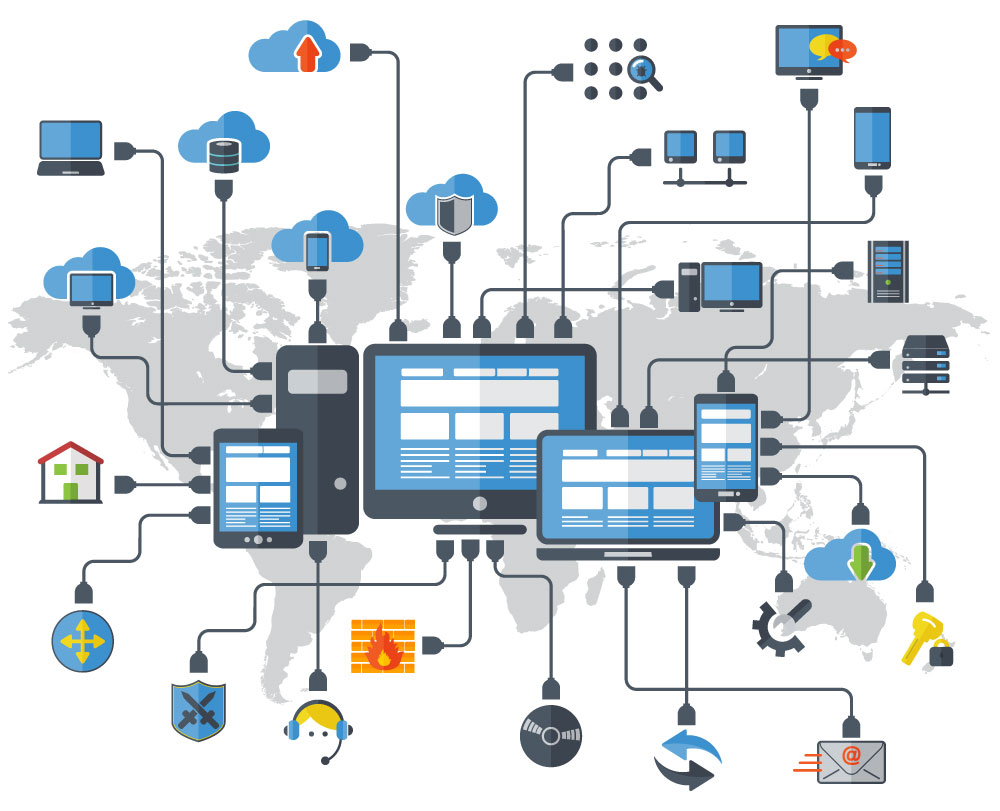
\includegraphics[height=3.6 in]{images/ATHENAnetsec.jpg}
\end{center}
\caption{ Network security }
\label{netsec}
\end{figure} 
As described in Figure \ref{netsec}, enterprises uses network to connect almost all of their components in each department or field finance, development, administration and sometimes from home or connected with clients, network is then critical as it guaranties access through equipment and personal data. Therefore, network security becomes a necessity because the control of access to files and directories is imperative against hacking, misuse and unauthorized changes to the system. Nowadays, some solutions may be integrated in companies like firewalls and anti-viruses, but is that really enough?  

\item\textbf{Monitoring}

Network monitoring can be many ways of recording traffic both ways inside the enterprise or outside the internet, those recordings changes format according to what product or solution is used. 
Even though some products controls access to enterprise's network, there is always a chance for attackers to gain access and bypass those implemented ways of protection, for that, monitoring network traffic in a company becomes useful to prevent breaches sometimes before it happens or later during investigation for it doesn't happen again. A couple of (free/payed) monitoring solutions is well known at the market like PRTG, NetworkMiner and other sniffers, but there is always a problem in those product either it is highly expensive or demands a lots of disk space and a group of analysts other than the community guidance that is often payed. 
\item\textbf{ IDS / IPS }

Intrusion Detection or prevention systems are network security appliances that monitor network or system activities for malicious activity. An Intrusion Detection System (IDS) is the process of monitoring the events occurring in your network and analyzing them for signs if possible incidents, violations or threatens your security policies. In the other hand Intrusion Prevention system is performing an IDS with the ability of stopping the detected incidents. IPS are often used because of the problems it may occurs to the enterprises for example stopping service(s) according to a false alarm(s). 
\begin{figure}[!htpb] 
\begin{center}
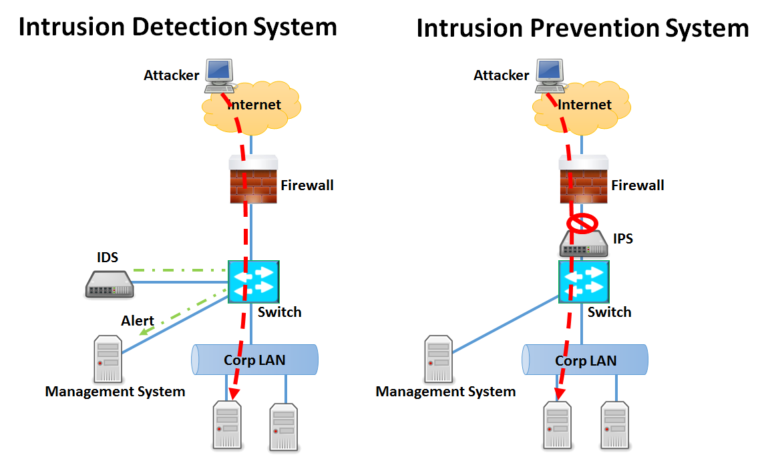
\includegraphics[height=3.6 in]{images/ATHENAidsips.png}
\end{center}
\caption{ IDS / IPS }
\label{idps}
\end{figure}


\item\textbf{Honeypots}

Honeypots are defined as decoy systems, their goal is to divert malicious traffic away from important systems, deployed alongside production systems with the intent of tricking hackers and gather information about intruders and guaranties early warning of a current attack before critical systems are hit. Those informations can be used for forensic or legal purposes.
\item\textbf{Threat intelligence}

In a military, business or security context, intelligence is information that provides an organization with decision support and possibly a strategic advantage. Threat intelligence is a component of security intelligence and includes both the information relevant to protecting an organization from external and inside threats as well as the processes, policies and tools designed to gather and analyze that information.
\end{itemize}
\subsection{Comparative analysis }
\subsubsection{ Intrusion Detection/Prevention Systems}
In the following comparison, three main point are compared (Performance, usage and Community)
\begin{itemize}[label=\ding{112}]
\item\textbf{Open-Source}

\begin{figure}[!htpb] 
\begin{center}
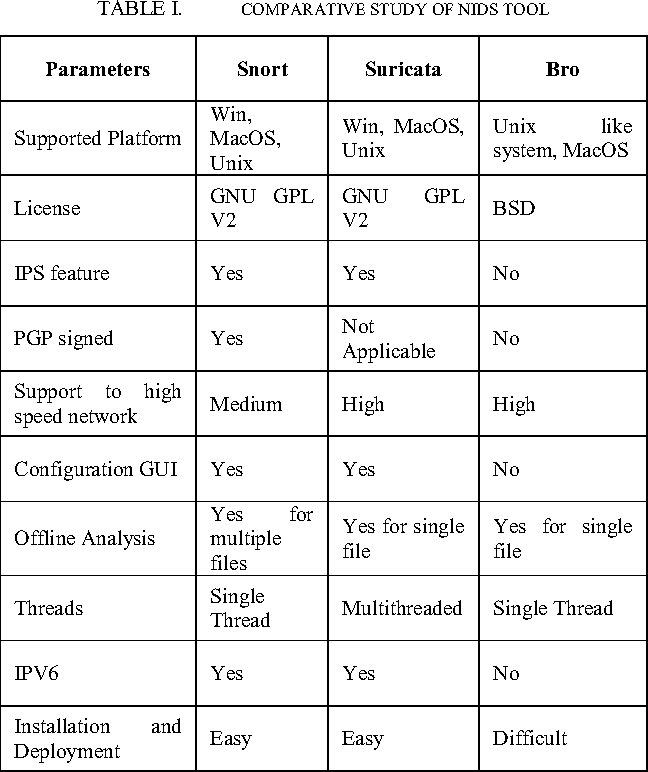
\includegraphics[height=3.8 in]{images/ATHENANIDS.png}
\end{center}
\caption{ Semantic Scholar Network IDS/IPS comparative analysis }
\label{nids}
\end{figure}
Snort , Suricata and Bro are the main three most powerful networks intrusion detection and/or prevention system in the world market. Based on the comparative analysis mentioned by Semantic scholar in Figure \ref{nids} and the test platform we performed : Snort is highly efficient in the scenario of moderate traffic with a single core processor. Based on architecture, snort uses 10 percent of CPU for parsing, 10 to 20 percent for normalization and 70 to 80 percent of CPU for payload inspection and detection. In a test performed by SANS, Snort gave a performance of 500Mbps with 1 CPU core for 1000 signatures. For 4000 signatures, it required 2.4 CPU at a rate of 400Mbps. It was found that a single instance of Snort is more efficient than Suricata with 50 percent less memory use. Recent versions of Snort support PF-RING and PCAP acceleration providing support for higher traffic. 

Suricata is more focused on large scale networks. In a way, it could be considered as an extension of Snort for large networks. In a scenario with a 45 CPU hosting 12 cores per CPU and 125 GB of RAM, the network throughput was 20 Gbps. Suricata had a very less packet drop of 7 percent while it was 53 percent in Snort. Suricata provides support for PF-Ring, AF packet, PCAP acceleration and NFLOG. It also works better with multi-threading. In snort the normalization is performed for every instance while for Suricata and Bro, the normalization is performed only once before multithreading. Suricata also support GPU cuda acceleration for pattern matching. There are also about 4000 file types build for file extraction and logging also providing MD5 matching. 

Bro as mentioned above is script driven IDS. Bro has support for clustering for high throughput environments. Bro provides a worker based architecture to use multiple processors. 
Bro’s developers recommend allocating one core for every 80 Mbps of traffic that is being analyzed.
It also have features allowing to interact with other systems in the enterprise, send email messages, page on-call staff, or automatically terminate existing connections. Bro also works based on file hash extraction and matching with the use of publicly available hash registers.
It is important to notice that the processing per core is significantly low compared to Snort or Suricata. But Bro has built in capacity to spread the load across multiple machines via Bro cluster thereby proving greater scalability. 
But there have some research showing that the overhead of distributed processing slows down the performance. Thus the performance acceleration is applicable only till a certain saturation point.

As for the usage, Suricata has a very similar rule set and configuration parameters to snort. While Bro could be called a behavior based one, with a very different approach compared to the idea of rules. Bro works with scripts. 

\begin{figure}[!htpb] 
\begin{center}

\includegraphics[height=1 in]{images/ATHENAnidss.png}
\end{center}
\caption{ Snort, Suricata and Bro logos }
\label{nidss}
\end{figure}

An IDS solution is only as good as the available rules it can apply to the monitored traffic. Snort has always had a lot of community support, and this has led to a substantial ruleset, updated on a regular basis. 

Suricata can use the same rules as SNORT. Many, but not all, VRT rules do still work. Suricata has its own ruleset, initially released to paying subscribers, but freely available after 30 to 60 days.

There is a number of resources available to provide help with using Bro, including channels to reach out the broader community and a commercial option for sites that need professional support.
\item\textbf{Paid Solutions}

Non Free products for intrusion detection or prevention systems are aften integrated with firewalls or Network Security Monitoring (NSM) tools, pre-configured by the provider and its support group for later charges in case of later modifications or re-configurations wanted by the client. An example of well known and trusted products are mentioned below:
\begin{itemize}
    \item Juniper Networks uses its SRX Series Services Gateways for intrusion detection and prevention (IDP) services. 

    \item McAfee uses its network threat and intrusion prevention solution Network Security Platform (NSP).
\end{itemize}

Since ATHENA is interested in new technologies and open-source products, while free open-source IDS and IPS software exists, these solutions often require an IT pro to make sure the IDS and IPS rules are up-to-date.

For a network such as ATHENA’s, it is more suitable to integrate Bro and Snort, as we can see with Bro’s great flexibility and Snort’s functionalities we can assume that nearly 100 percent of anomalies should be detected and reported.

\end{itemize}
\subsubsection{ SIEM }
\begin{figure}[!htpb] 
\begin{center}
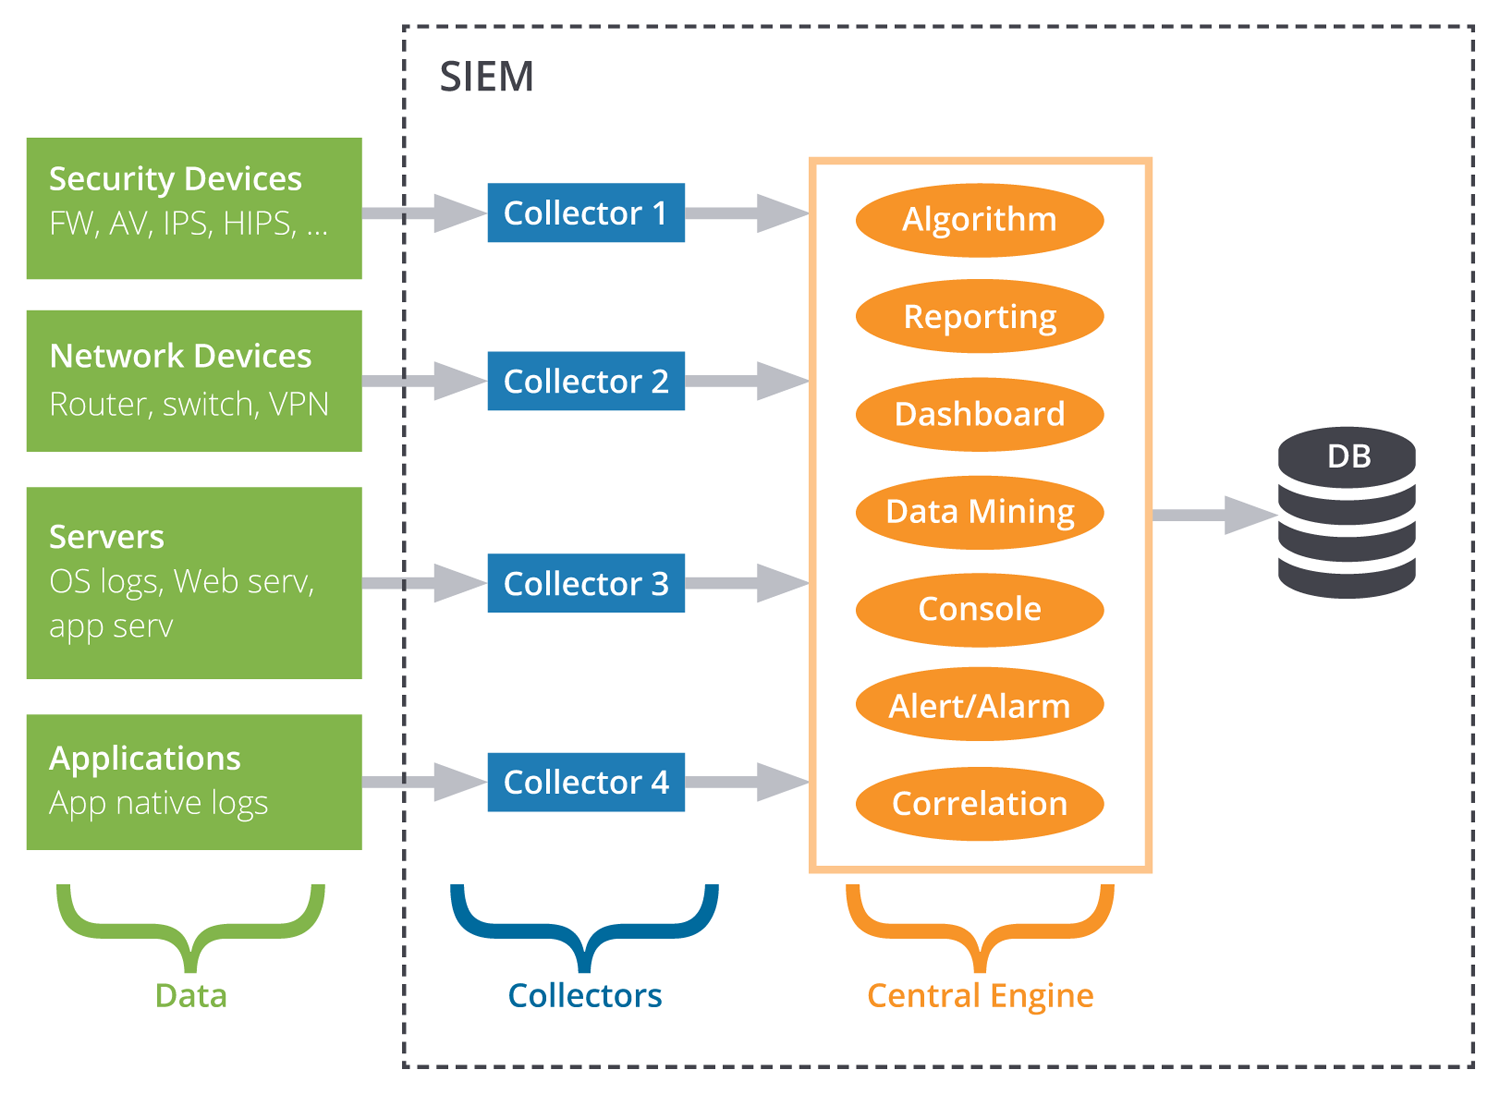
\includegraphics[height=3.0 in]{images/ATHENAsiem.png}
\end{center}
\caption{ Security information and event management }
\label{siem}
\end{figure}
Security information and event management (SIEM) is as mentioned in Figure \ref{siem}, a combination between security information management (SIM) and security event management (SEM). A centralized management platform of security events and alerts.
We focused on the the two main powerful solution in the world market according to test result of both solutions and user experience, Splunk and ELK :

\begin{itemize}
    \item ELK 
    
    It's a free open-source combination between ElasticSearch which is distributed, RESTful, JSON-based search engine. Easy to use, scalable and flexible. Logstash the powerful ingest pipeline and Kibana the flexible visualization tool. The Elastic Stack is loved by developers, From the perspective of the technical staff at Search Technologies, however, getting up to speed on ELK was relatively easy. They commented that the developer experience is also very good.
    \item Splunk
    
    Splunk Still Rules the Log Analytics Market for log analytics applications, and with over 500 million Dollars in revenues, Splunk is still the undisputed market leader. 
\begin{figure}[!htpb] 
\begin{center}
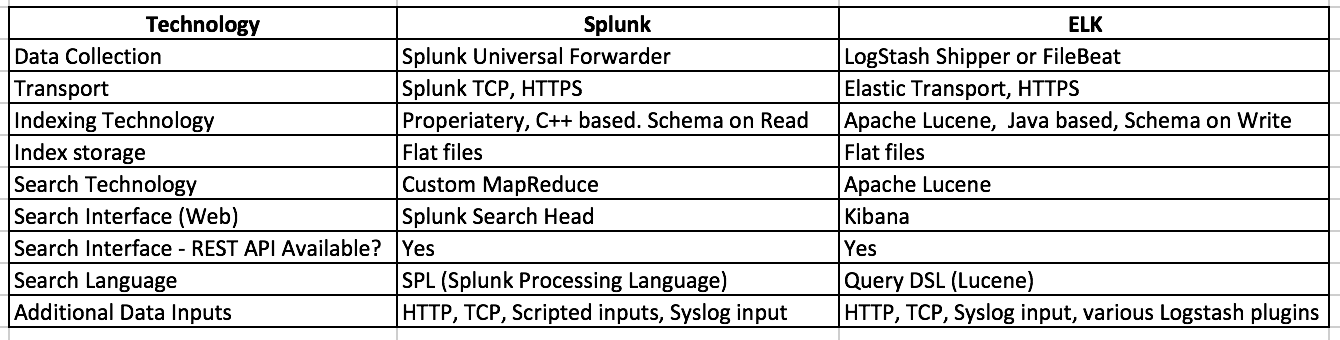
\includegraphics[width=18cm]{images/ATHENAsiemcompare.png}
\end{center}
\caption{ SIEM Comparative analysis }
\label{siemcomp}
\end{figure}

As in Figure \ref{siemcomp}, splunk and Elastic Stack are technically different.
In short, both Splunk and ELK/Elastic Stack are competent, enterprise-grade log management and analysis platforms trusted by the world's leading organizations. Total cost of ownership can be significant for both solutions; in response to demand from more budget-minded firms, Splunk and Elastic have recently started to offer hosted versions of their products. 

\end{itemize}
\subsubsection{ Security Monitoring Operating systems}

A network security monitoring toolkit has been always an interest to all enterprises, therefore some solutions already runs the market, in this section we are going to compare some of the most powerful security monitoring open-source solutions 

\begin{itemize}[label=\ding{112}]
\item\textbf{SELKS}

An Optimized hardware and multi layered Linux based operating system(both Live and installable Network Security Management ISO based on Debian) developed by Stamus Networks, the French company with headquarters in Paris who  believes in the innovative power and flexibility that Open Source Software posses. 
SELKS is combination of Suricata as its intrusion detection system, ELK as its SIEM and Scirius as a web management interface for Suricata rules and alerts, SELKS is currently running with a stable version 4.0 and as it shows in Figure \ref{selks}, it guaranties the following features :
\begin{itemize}
    \item Intrusion Detection System with ETPRO ruleset and your company/site/department specific rules.
    \item Web management interface: ruleset, config parameters.
    \item Log analysis via a scalable Elasticsearch with real time search and drill-down approach.
    \item Container: GNU/Linux distributions to run any task on Suricata generated data (IOC, connection to the SIEM).
    \item Network Security Monitoring: HTTP, DNS, TLS, SSH, File extraction, alert logging and many more.
    \item Proven 10+ Gbps full inspection.
    \item Enterprise support.
    \item Multi probe/Multi site scalable deployment.
\end{itemize}

\begin{figure}[!htpb] 
\begin{center}
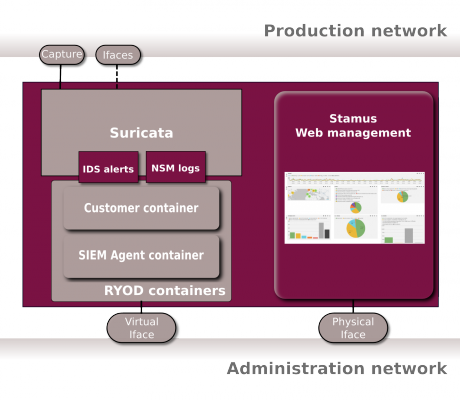
\includegraphics[height=3.6 in]{images/ATHENAselks.png}
\end{center}
\caption{ SELKS }
\label{selks}
\end{figure}

\item\textbf{SecurityOnion}

Security Onion is a free and open source Linux distribution maintained by Doug Burks  for intrusion detection, enterprise security monitoring, and log management. It includes Elasticsearch, Logstash, Kibana, Snort, Suricata, Bro, OSSEC, Sguil, Squert, NetworkMiner, and many other security tools. The easy-to-use Setup wizard allows you to build an army of distributed sensors for your enterprise. 

Security Onion seamlessly weaves together three core functions:
    \begin{itemize}
        \item Full packet capture.
        \item Network-based and host-based intrusion detection systems (NIDS and HIDS, respectively).
        \item and powerful analysis tools.
    \end{itemize}

Network-based and host-based intrusion detection systems (IDS) analyze network traffic or host systems, respectively, and provide log and alert data for detected events and activity. Security Onion provides multiple IDS options:
    \begin{itemize}
        \item\textbf{Rule-driven NIDS}
        
        For rule-driven network intrusion detection, Security Onion offers the choice of Snort or Suricata.
        \item\textbf{Analysis-driven NIDS}
        
        For analysis-driven network intrusion detection, Security Onion offers The Bro Network Security Monitor, also known as Bro IDS.
    \end{itemize}
For host-based intrusion detection, Security Onion offers OSSEC, a free, open source HIDS for Windows, Linux and Mac OS X. When you add the OSSEC agent to endpoints on your network, you gain invaluable visibility from endpoint to your network’s exit point. 
\begin{figure}[!htpb] 
\begin{center}
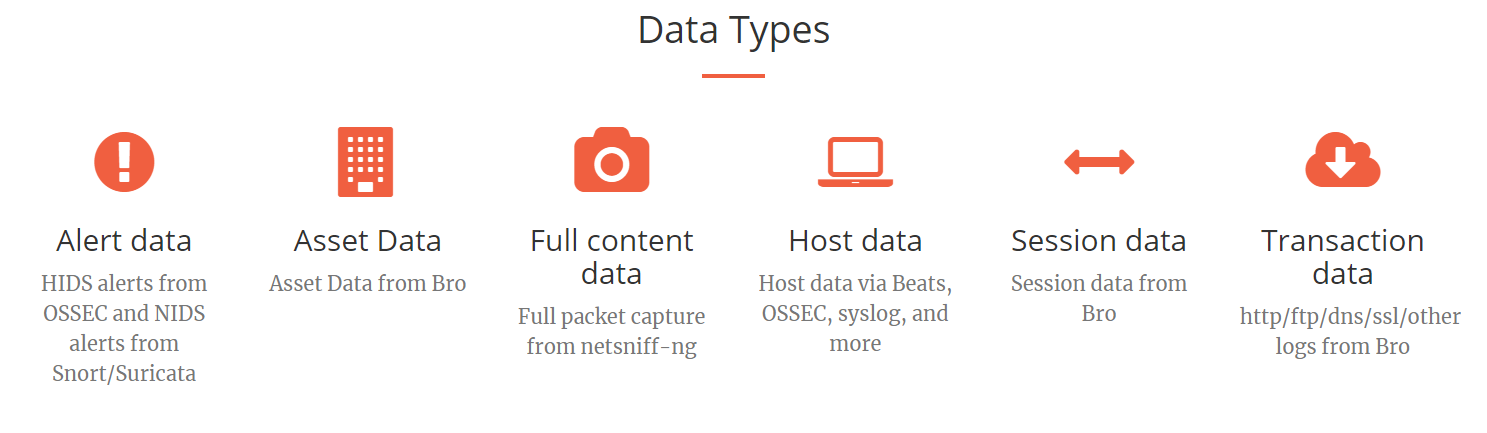
\includegraphics[width=18 cm]{images/ATHENAsoso.png}
\end{center}
\caption{ SecurityOnion Retrievable Data types }
\label{so}
\end{figure}
With full packet capture, IDS logs and Bro data, there is a daunting amount of data available at the analyst’s fingertips. Fortunately, Security Onion integrates the following tools to help make sense of this data:
    \begin{itemize}
        \item\textbf{Sguil} 
        
        Created by Bamm Visscher (@bammv), is “The Analyst Console for Network Security Monitoring.” It is the analyst’s right hand, providing visibility into the event data being collected and the context to validate the detection. Sguil provides a single GUI (written in tcl/tk) in which to view Snort or Suricata alerts, OSSEC alerts, Bro HTTP events, and Passive Real-Time Asset Detection System (PRADS) alerts. More importantly, Sguil allows you to “pivot” directly from an alert into a packet capture (via Wireshark or NetworkMiner) or a transcript of the full session that triggered the alert.
        
        \item\textbf{Squert}
        
        Created by Paul Halliday (@01110000), is a web application interface to the Sguil database. Although it is neither meant to be a real-time (or near real-time) interface nor a replacement for Sguil, it allows querying of the Sguil database and provides several visualization options for the data such as “time series representations, weighted and logically grouped result sets” and geo-IP mapping.
\end{itemize}


Security Onion is built on a distributed client-server model. A Security Onion “sensor” is the client and a Security Onion “server” is, well, the server. The server and sensor components can be run on a single physical machine or virtual machine, or multiple sensors can be distributed throughout an infrastructure and configured to report back to a designated server. An analyst connects to the server from a client workstation (typically a Security Onion virtual machine installation) to execute queries and retrieve data.
The following are the three Security Onion deployment scenarios:
    \begin{itemize}
    \item\textbf{Standalone:}
    
    A standalone installation consists of a single physical or virtual machine running both the server and sensor components and related processes. 
    \item\textbf{Server-sensor:}
    
    A server-sensor installation consists of a single machine running the server component with one or more separate machines running the sensor component and reporting back to the server.
    \item\textbf{Hybrid:}
    
    A hybrid installation consists of a standalone installation that also has one or more separate sensors reporting back to the server component of the standalone machine.
    \end{itemize}

\end{itemize}


%%%%%%%%%%%%%%%%%%%%%%%%%%%%%%%%%%%%%%%%%%%%%%%%%%%%%%%%%%%%%%%%%%%%%%%
%%%%%%%%%%%%%%%%%%%%%%%%%%%%%%%%%%%%%%%%%%%%%%%%%%%%%%%%%%%%%%%
\ifx
SaaS cloud level is usually a catalog of applications available as a service to end users or customers.
In other words, this level offers a range of services "modable" and "customizable". It may be noted as an example a courier, CMS, access to libraries, shopping in online stores etc.
Using this mode is also useful when prototyping phase in a short time and at low cost.

Cloud service models Cloud Computing as general term sits over a variety of services
from Infrastructure as a Service at the base, through Platform as a Service as a development
tool and through to Software as a Service replacing on-premise applications.

Software as a Service (SaaS): SaaS is the highest level. At this level, the capability
provided to the consumer is to use the provider’s applications running on a cloud infrastructure.
The applications are accessible from various client devices through either
a thin client interface, such as a web browser (e.g., web-based email), or a program interface.
The consumer does not manage or control the underlying cloud infrastructure including network, servers, operating systems, storage, or even individual application capabilities, with the possible exception of limited user-specific application configuration settings.[B1]

\item\textbf{SPA }

A Single Page Application is a web developed application that can be displayed on a single web page in order to simulate the desktop application experience for users.
As the developers see it fit, it can either retrieve the necessary source code with one single page load, or dynamically load the necessary resources in response to the user requirements. The page in question does not reload at any point of the process nor modulate the data communication with other pages.


\item\textbf{Google Maps API }

Google provides many special-purpose APIs. The use of this specific API is mandatory while building a geolocalization application.
This part highlights the capability of Google map API.

It is a Google Application Programming Interface that handles the geolocalization of an address granted its latitude and longitude and spotting it on the map.
The Api provides multiple services such as mapping data display which offers Internet users a global geographic data vision. 

The data displayed on the map is dressed up as a pictogram: small clickable items. Once clicked, the icon leads to a set of information concerning the geolocalized data. 
It is also possible to set an itinerary by assigning the starting point and the destination which would generate a time estimation for each proposed itinerary.
It is also possible to calculate a route (pedestrian or car) from a starting point  to a point of arrival.[B2]
\fi


\ifx
\subsection{AJAX }
Ajax is a set of programming techniques or a particular approach to web programming. 
These programming techniques involve being able to seamlessly update a web page or a section of a web application with input from the server, but without the need for an immediate page refresh. This does not mean that the browser does not make a connection to the web server.

\begin{figure}[!htpb] 
\begin{center}
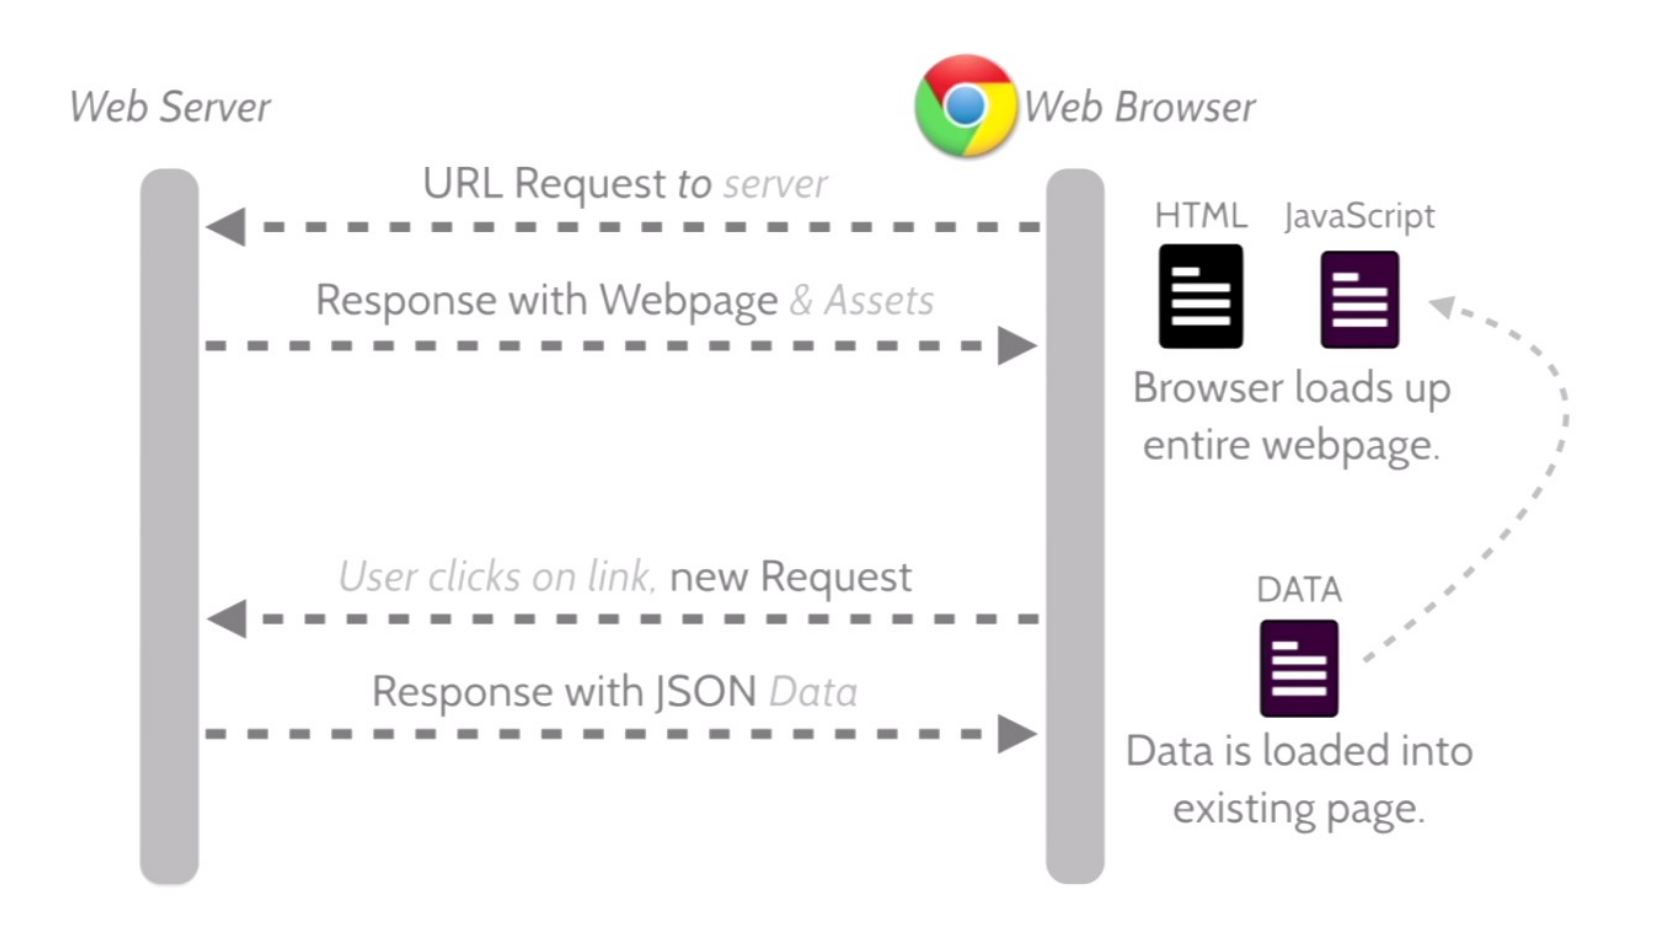
\includegraphics[height=3.6 in]{images/ajax2.png}
\end{center}
\caption{« AJAX » application }
\label{ajax}
\end{figure} 

Figure \ref{ajax} [B3] demonstrates how AJAX works. It allows web pages to be updated
asynchronously by exchanging small amounts of data with the server behind the scenes. This means that it is possible to update parts of a web page, without reloading the whole page. 
Classic web pages, (which do not use AJAX) must reload the entire page if the content should change. Examples of applications using AJAX: Google Maps, Gmail, Youtube, and Facebook tabs.
We explain and enumerate which technologies related to AJAX are incorporated in
the development of our application:

\begin{itemize}
    
    \item HTML (or XHTML) and CSS for presentation (to mark up and style the data).
    
    \item The HTML DOM defines a standard set of objects for HTML, and a standard way to access
and manipulate HTML documents. The utility of DOM is that all HTML elements, along with
their containing text and attributes, can be accessed through it. Their contents can be modified or deleted, and new elements can be created. DOM can be used by any programming language like
Java, JavaScript, and VBScript \cite{w3school}. In our Case we used it especially to manipulate the elements of the user interface.
Document Object Model (DOM) is accessed with JavaScript for dynamic display and
interaction with data. 


\item JSON is designed to be a data interchange format which is human readable and easy for computers to parse and use. JSON is directly supported inside JavaScript and is best suited for JS applications; thus providing significant performance gains over XML, which requires extra libraries to retrieve data from Document Object Model (DOM) objects. JSON is estimated to parse up to one hundred times faster than XML in modern browsers.Validation of inputs is the responsibility of individual domain applications, and the lack of extensibility claims is addressed by the flexibility of JSON constructs. \cite{json} The next lines describe an example of JSON to clarify its structure.

\{ "firstname" : "John",

"lastname" : "Smith" \}

\item JavaScript to bring these technologies together.

\end{itemize}
\fi %%%%%%%%%%%%%%%%%%%%%%%%%%%%%%%%%%%%%%%%%%%%%%%%%%%%%%%%%%%%%%%%% %%%%%%%%%%%%%%%%%%%%%%%%%%%%%%%%%%%%%%%%%%%%%%%%%%%%%%%%%%%%%%%

%--------------------------------------------------Study of existing and critics  & proposed solution


\section{Study of the solution}
~~~In this part, we describe briefly the solution already implemented and criticize its drawbacks. After that, we present the advantages of our proposed component.

As evoked in the previous chapter, the solution is a network security monitoring toolkit that offers services to complete a security operation center.

\subsection{ATHENA's network}

As the number of servers and services increases, it is becoming more and more challenging to control and observe the traffic passing by them all. Figure \ref{networkarch} exhibit the network architecture of ATHENA. 

~

\begin{figure}[!htpb]
\begin{center}
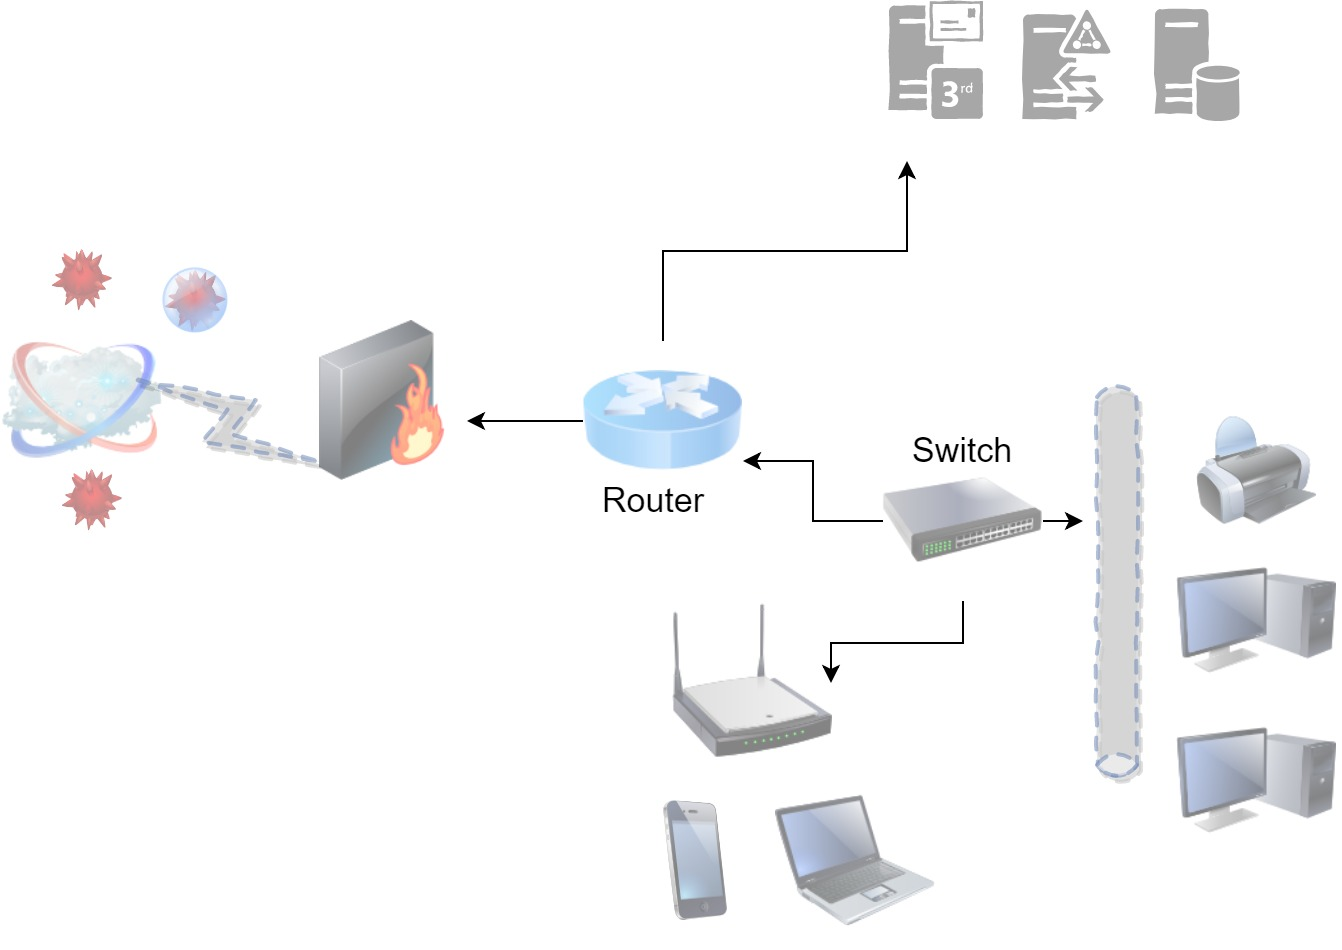
\includegraphics[height=3.5 in]{images/ATHENAnetw.jpg}
\caption{ATHENA's Network general view}
\label{networkarch}
\end{center}
\end{figure} 

Server are placed separately from the private network for security reasons, the private network is divided between physical and wireless connections, user's permissions are managed through vlans. An ASA firewall is well configured to prevent and control access from the outside.
\subsection{Proposed solution}

Based on the previous state of network in ATHENA, The major features of our solution should be:

\begin{itemize}
    \item Sensor or probe to monitor the traffic coming in and out both private and demilitarized zone.
    \item Incident response mechanism to report alerts.
    \item Visualization platform for analysts.
    \item Threat intelligence platform.
    \item Honeynet (Centralized management of Honeypots) to trick attackers and gather information about intruders.
    \item Servers and services monitoring.
    \item Management interface for analysts to control and deploy sensors.
\end{itemize}


~





%---------------------------------------------------------conclusion
\subsection *{Conclusion}
In this chapter, we went through a brief study of the state of the art while presenting the most important concepts used in this project. After that, we reviewed the existing solution and we highlighted our contribution.
In the next chapter, we enumerate the different features offered by our application and we present the main possible scenarios.
